\documentclass{beamer}

\usepackage{listings}  % Package to include python syntax code
\usepackage{color} % Package to include colors for syntax highlighting
\usepackage{graphicx}  % Package to include images
\usepackage{hyperref}  % Hyperlinks
\usepackage{tikz}

\lstset{  % Settings for listings package
backgroundcolor=\color{cyan!10},  % Includes a light blue background color
numbers=left,  % Includes line numbers
keywordstyle=\bfseries\color{green!40!black},  % Bold and color green for keywords
identifierstyle=\color{blue},  % Other words are colored blue
stringstyle=\color{orange},  % Strings are orange
showstringspaces=false  % Don't show spaces in strings
}

\setbeamertemplate{navigation symbols}{}  % Remove navigation symbols

\title{Computing for Mathematics: Second Semester}
\date{}


\begin{document}

\frame{
\titlepage
}

\frame{
\frametitle{Vince Knight}
\begin{itemize}
    \item Office: M1.30
    \item email: knightva@cf.ac.uk
    \item Office hours: Thursday 1300 - 1500
\end{itemize}
}

\frame{
\frametitle{Coursework}

\begin{center}
\only<1>{
\includegraphics[width=.8\textwidth]{/Users/vince/Dropbox/Shared/CfM2013Marking/indcwmarkdistribution.pdf}
}
\only<2>{
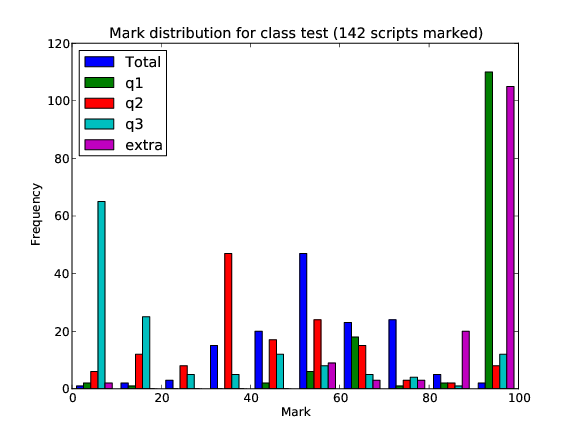
\includegraphics[width=.8\textwidth]{/Users/vince/Dropbox/Shared/CfM2013Marking/markdistribution.pdf}
}
\end{center}
}

\frame{\frametitle{Prizes}
\pause
\begin{itemize}
    \item Mathew Lunn: Prime Number Theorem;\pause
    \item Alex Carney: Fractals;\pause
    \item James Campbell: Python and Ladders.
\end{itemize}
}

\frame{\frametitle{Conference}
\begin{center}
\url{https://djangoweekend.org/}
\end{center}
}

\frame{\frametitle{The Next 11 weeks}
\begin{center}
    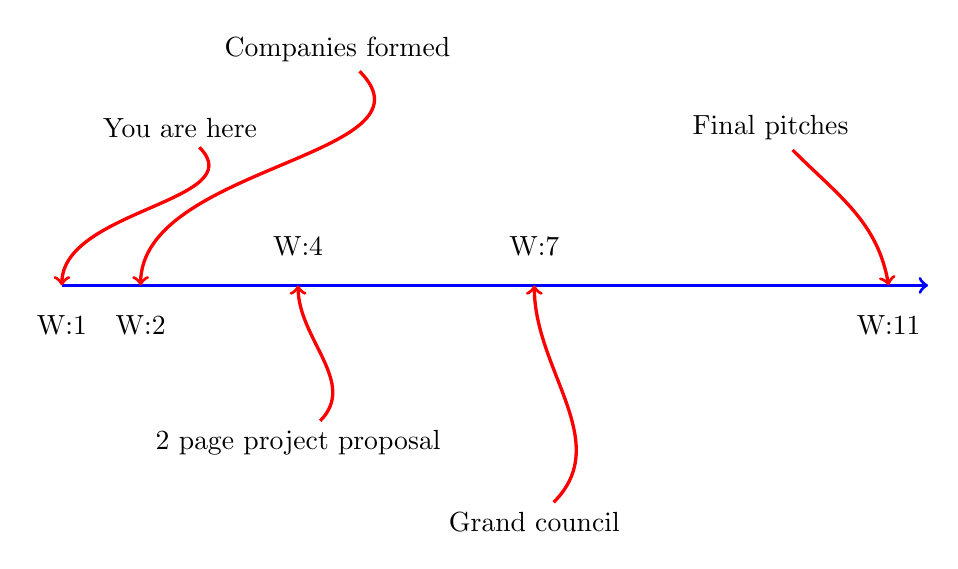
\begin{tikzpicture}
        \draw (0,0) edge[very thick, blue, ->] (11,0);
        \pause
        \node (A) at (1.5,2) {You are here};
        \draw (A) edge[out=-45, in=90, ->, very thick, red] (0,0);
        \node at (0,-.5) {W:1};
        \pause
        \node (B) at (3.5,3) {Companies formed};
        \draw (B) edge[out=-45, in=90, ->, very thick, red] (1,0);
        \node at (1,-.5) {W:2};
        \pause
        \node (C) at (3,-2) {2 page project proposal};
        \draw (C) edge[out=45, in=-90, ->, very thick, red] (3,0);
        \node at (3,.5) {W:4};
        \pause
        \node (D) at (6,-3) {Grand council};
        \draw (D) edge[out=45, in=-90, ->, very thick, red] (6,0);
        \node at (6,.5) {W:7};
        \pause
        \node (E) at (9,2) {Final pitches};
        \draw (E) edge[out=-45, in=100, ->, very thick, red] (10.5,0);
        \node at (10.5,-.5) {W:11};
    \end{tikzpicture}
\end{center}
}

\frame{\frametitle{Companies}
\begin{itemize}
    \item Groups of 4:
        \begin{itemize}
            \item Company Director;
            \item Company Secretary.
        \end{itemize}
    \item You are expected to meet \textbf{at least once a week}!
    \item \textbf{Minutes of meetings (1 page) to be handed in every week}!
\end{itemize}
}

\frame{\frametitle{Group Work}
\begin{center}
    \includegraphics[height=.8\textheight]{/Users/vince/Desktop/groupwork.jpg}
\end{center}
}

\frame{\frametitle{Next Deadlines}
\begin{itemize}
    \item From groups: \textbf{immediately};
    \item Minutes: next Lecture;
    \item Project proposal (2 page document): \textbf{20th of February}.
\end{itemize}
}

\frame{\begin{center}
\Huge{Neil Coles}
\end{center}}

\end{document}
